%!TEX TS-program = xelatex
\documentclass[12pt, a4paper, oneside]{article}

% Можно вставить разную преамбулу
% пакеты для математики
\usepackage{amsmath,amsfonts,amssymb,amsthm,mathtools}  
\mathtoolsset{showonlyrefs=true}  % Показывать номера только у тех формул, на которые есть \eqref{} в тексте.

\usepackage[british,russian]{babel} % выбор языка для документа
\usepackage[utf8]{inputenc}          % utf8 кодировка

% Основные шрифты 
\usepackage{fontspec}         
\setmainfont{Linux Libertine O}  % задаёт основной шрифт документа

% Математические шрифты 
\usepackage{unicode-math}     
\setmathfont[math-style=upright]{euler.otf} 

\setmathfont[range={\mathbb, \mathop, \heartsuit, \angle, \smile, \varheartsuit}]{Asana-Math.otf}

%%%%%%%%%% Работа с картинками и таблицами %%%%%%%%%%
\usepackage{graphicx} % Для вставки рисунков                
\usepackage{graphics}
\graphicspath{{images/}{pictures/}}   % папки с картинками

\usepackage[figurename=Картинка]{caption}

\usepackage{wrapfig}    % обтекание рисунков и таблиц текстом

\usepackage{booktabs}   % таблицы как в годных книгах
\usepackage{tabularx}   % новые типы колонок
\usepackage{tabulary}   % и ещё новые типы колонок
\usepackage{float}      % возможность позиционировать объекты в нужном месте
\renewcommand{\arraystretch}{1.2}  % больше расстояние между строками


%%%%%%%%%% Графики и рисование %%%%%%%%%%
\usepackage{tikz, pgfplots}  % языки для графики
%\pgfplotsset{compat=1.16}

\usepackage{todonotes} % для вставки в документ заметок о том, что осталось сделать
% \todo{Здесь надо коэффициенты исправить}
% \missingfigure{Здесь будет Последний день Помпеи}
% \listoftodos --- печатает все поставленные \todo'шки

\usepackage{multicol}

%%%%%%%%%% Внешний вид страницы %%%%%%%%%%

\usepackage[paper=a4paper, top=20mm, bottom=15mm,left=20mm,right=15mm]{geometry}
\usepackage{indentfirst}    % установка отступа в первом абзаце главы

\usepackage{setspace}
\setstretch{1.15}  % межстрочный интервал
\setlength{\parskip}{4mm}   % Расстояние между абзацами
% Разные длины в LaTeX: https://en.wikibooks.org/wiki/LaTeX/Lengths

% свешиваем пунктуацию
% теперь знаки пунктуации могут вылезать за правую границу текста, при этом текст выглядит ровнее
\usepackage{microtype}

% \flushbottom                            % Эта команда заставляет LaTeX чуть растягивать строки, чтобы получить идеально прямоугольную страницу
\righthyphenmin=2                       % Разрешение переноса двух и более символов
\widowpenalty=300                     % Небольшое наказание за вдовствующую строку (одна строка абзаца на этой странице, остальное --- на следующей)
\clubpenalty=3000                     % Приличное наказание за сиротствующую строку (омерзительно висящая одинокая строка в начале страницы)
\tolerance=10000     % Ещё какое-то наказание.

% мои цвета https://www.artlebedev.ru/colors/
\definecolor{titleblue}{rgb}{0.2,0.4,0.6} 
\definecolor{blue}{rgb}{0.2,0.4,0.6} 
%\definecolor{red}{rgb}{1,0,0.2} 
\definecolor{green}{rgb}{0, 0.6, 0}
\definecolor{purp}{rgb}{0.4,0,0.8} 

\definecolor{red}{RGB}{213,94,0}
\definecolor{yellow}{RGB}{240,228,66}


% цвета из geogebra 
\definecolor{litebrown}{rgb}{0.6,0.2,0}
\definecolor{darkbrown}{rgb}{0.75,0.75,0.75}

% Гиперссылки
\usepackage{xcolor}   % разные цвета

\usepackage{hyperref}
\hypersetup{
	unicode=true,           % позволяет использовать юникодные символы
	colorlinks=true,       	% true - цветные ссылки
	urlcolor=blue,          % цвет ссылки на url
	linkcolor=black,          % внутренние ссылки
	citecolor=green,        % на библиографию
	breaklinks              % если ссылка не умещается в одну строку, разбивать её на две части?
}

% меняю оформление секций 
\usepackage{titlesec}
\usepackage{sectsty}

% меняю цвет на синий
\sectionfont{\color{titleblue}}
\subsectionfont{\color{titleblue}}

% кружочки у цифр в секциях
\renewcommand{\thesection}{\arabic{section}}

% https://ru.overleaf.com/learn/latex/Sections_and_chapters

% выбрасываю нумерацию страниц и колонтитулы 
%\pagestyle{empty}

% синие круглые бульпоинты в списках itemize 
\usepackage{enumitem}

\definecolor{itemizeblue}{rgb}{0, 0.45, 0.70}

\newcommand*{\MyPoint}{\tikz \draw [baseline, fill=itemizeblue, draw=blue] circle (2.5pt);}
\renewcommand{\labelitemi}{\MyPoint}

\AddEnumerateCounter{\asbuk}{\@asbuk}{\cyrm}
\renewcommand{\theenumi}{\asbuk{enumi}}

% расстояние в списках
\setlist[itemize]{parsep=0.4em,itemsep=0em,topsep=0ex}
\setlist[enumerate]{parsep=0.4em,itemsep=0em,topsep=0ex}

% эпиграфы
\usepackage{epigraph}
\setlength\epigraphwidth{.6\textwidth}
\setlength\epigraphrule{0pt}

%%%%%%%%%% Свои команды %%%%%%%%%%

% Математические операторы первой необходимости:
\DeclareMathOperator{\sgn}{sign}
\DeclareMathOperator*{\argmin}{arg\,min}
\DeclareMathOperator*{\argmax}{arg\,max}
\DeclareMathOperator{\Cov}{Cov}
\DeclareMathOperator{\Var}{Var}
\DeclareMathOperator{\Corr}{Corr}

\DeclareMathOperator{\Pois}{Pois}
\DeclareMathOperator{\Geom}{Geom}
\DeclareMathOperator{\Exp}{Exp}

%\DeclareMathOperator{\E}{\mathbb{E}}
\DeclareMathOperator{\Med}{Med}
\DeclareMathOperator{\Mod}{Mod}
\DeclareMathOperator*{\plim}{plim}

% команды пореже
\newcommand{\const}{\mathrm{const}}  % const прямым начертанием
\newcommand{\iid}{\sim i\,i\,d\,\,}  % ну вы поняли...
\newcommand{\fr}[2]{\ensuremath{^{#1}/_{#2}}}   % особая дробь
\newcommand{\ind}[1]{\mathbbm{1}_{\{#1\}}} % Индикатор события
\newcommand{\dx}[1]{\,\mathrm{d}#1} % для интеграла: маленький отступ и прямая d

% одеваем шапки на частые штуки
\def \hb{\hat{\beta}}
\def \hs{\hat{s}}
\def \hy{\hat{y}}
\def \hY{\hat{Y}}
\def \he{\hat{\varepsilon}}
\def \hVar{\widehat{\Var}}
\def \hCorr{\widehat{\Corr}}
\def \hCov{\widehat{\Cov}}

% Греческие буквы
\def \a{\alpha}
\def \b{\beta}
\def \t{\tau}
\def \dt{\delta}
\def \e{\varepsilon}
\def \ga{\gamma}
\def \kp{\varkappa}
\def \la{\lambda}
\def \sg{\sigma}
\def \tt{\theta}
\def \Dt{\Delta}
\def \La{\Lambda}
\def \Sg{\Sigma}
\def \Tt{\Theta}
\def \Om{\Omega}
\def \om{\omega}

% Готика
\def \mA{\mathcal{A}}
\def \mB{\mathcal{B}}
\def \mC{\mathcal{C}}
\def \mE{\mathcal{E}}
\def \mF{\mathcal{F}}
\def \mH{\mathcal{H}}
\def \mL{\mathcal{L}}
\def \mN{\mathcal{N}}
\def \mU{\mathcal{U}}
\def \mV{\mathcal{V}}
\def \mW{\mathcal{W}}

% Жирные буквы
\def \mbb{\mathbb}
\def \RR{\mbb R}
\def \NN{\mbb N}
\def \ZZ{\mbb Z}
\def \PP{\mbb{P}}
\def \E{\mbb{E}}
\def \QQ{\mbb Q}

\def\F{\ensuremath{\mathcal{F}}} % аналогично!

%%%%%%%%%% Теоремы %%%%%%%%%%
\theoremstyle{plain} % Это стиль по умолчанию.  Есть другие стили.
\newtheorem{theorem}{Теорема}[section]
\newtheorem{proposition}{Утверждение}[section]
\newtheorem{result}{Следствие}[section]

% убирает курсив и что-то еще наверное делает ;)
\theoremstyle{definition}         
\newtheorem*{definition}{Определение}  % нумерация не идёт вообще


%%%%%%%%%% Задачки и решения %%%%%%%%%%
\usepackage{etoolbox}    % логические операторы для своих макросов
\usepackage{environ}
\newtoggle{lecture}

\newcounter{probNum}[section]  % счётчик для упражнений 
\NewEnviron{problem}[1]{%
    \refstepcounter{probNum}% увеличели номер на 1 
    {\noindent \textbf{\large \color{titleblue} Упражнение~\theprobNum~#1}  \\ \\ \BODY}
    {}%
  }

% Окружение, чтобы можно было убирать решения из pdf
\NewEnviron{sol}{%
  \iftoggle{lecture}
    {\noindent \textbf{\large Решение:} \\ \\ \BODY}
    {}%
  }
 
% выделение по тексту важных вещей
\newcommand{\indef}[1]{\textbf{ \color{green} #1}} 

% разные дополнения для картинок
\usetikzlibrary{arrows.meta}
\usepackage{varwidth}

\usepackage[normalem]{ulem}  % для зачекивания текста

% Если переключить в false, все solution исчезнут из pdf
\toggletrue{lecture}
%\togglefalse{lecture}



\title{
\begin{center} 
\includegraphics[width=0.99\textwidth]{logo.png}
\end{center}

Посиделка 1: схема статистики}
\date{ } %\today}

% Если делаешь конспект, вписывай своё имя прямо сюда!
\author{Ульянкин Ппилиф}

\begin{document} % Конец преамбулы, начало файла

\maketitle

\epigraph{Уважаемые Знатоки, внимание вопрос: что в чёрном ящике?}{\textit{Господин Ведущий про интерпретируемость нейросетей}}


В этой лекции мы поговорим про то, зачем вы учили тервер. Мы обсудим как с помощью него можно замоделировать своё невежество и попытаться найти ответы на вопросы, которые нас мучают. Обсудим проверку гипотез и построим несколько простых критериев, основанных на комбинаторике.

\section{Зачем вы учили тервер}

Зачем вы изучали теорию вероятностей? Вам на ней говорили, что наша жизнь полна случайностей, а теория вероятностей помогает их описать. Например, вам говорили, что есть казино. В нём есть рулетка. Шарик катится по ней и выпадает какое-то число. Результат случаен. 

На самом деле это \indef{субъективная случайность.} При желании и технической оснащённости можно попытаться рассчитать, с какой именно скоростью шарик падает на рулетку, скорректировать его падение на то, как именно рулетка крутится, учесть ещё кучу разных факторов вроде скорости ветра и момента вращения, и у нас идеально получится предсказать куда именно упадёт шарик. Тем не менее, мы это не делаем, потому что у нас нет таких мощных вычислительных средств. Мы говорим, что падение шарика --- случайно, а \indef{вероятность описывает наше невежество.}

Точно также неслучайно то время, через которое автобус приедет на остановку. У нас нет никакой информации, что произошло с автобусом  на прошлой остановке и сколько он будет добираться до нашей. Во время его движения может столько всего произойти, и из-за того, что всего этого невозможно учесть, мы говорим, что время его приезда случайно.

Здесь можно подумать, что \indef{объективной случайности} в природе просто-напросто не существует, однако это не так. Объективная случайность наблюдается в квантовой физике (по крайней мере на нашем современном уровне её понимания), она вшита в наше естество на атомном уровне. 

Более того, если существует свобода воли (а это не факт), вряд ли получится предсказать, что именно взбредёт человеку сделать в следующую секунду, даже обладая самыми совершенными измерительными приборами. Можно рискнуть сказать, что поведению людей свойственна объективная неопределённость\footnote{Возможно, наше будущее предопределено, но человек не может этого осознать, и у него возникает ощущение, что он на что-то влияет. В таком случае свобода воли порождается субъективным незнанием, а не объективной неопределённостью. В фильме Прибытие (2016) как раз обыгрывается то, что у нас нет органа, который чувствовал бы будущее и из-за этого эволюционного невежества возникает иллюзия свободы воли.}.

Теория вероятности пытается предложить нам инструменты, которые помогут нам описать своё невежество с помощью субъективных случайностей. На ней вы изучили несколько моделей, которые можно использовать на практике для того, чтобы принимать решения и лучше понимать как всё работает. 

Весь наш мир --- это сундук. Мы не знаем, как он устроен. Он выплёвывает на нас данные. Посмотрев на эти данные, мы можем предположить как устроены внутренности сундука. Наше предположение --- это модель. Модели помогают нам принимать решения и предсказывать, что сундук выплюнет на нас дальше.

\begin{center} 
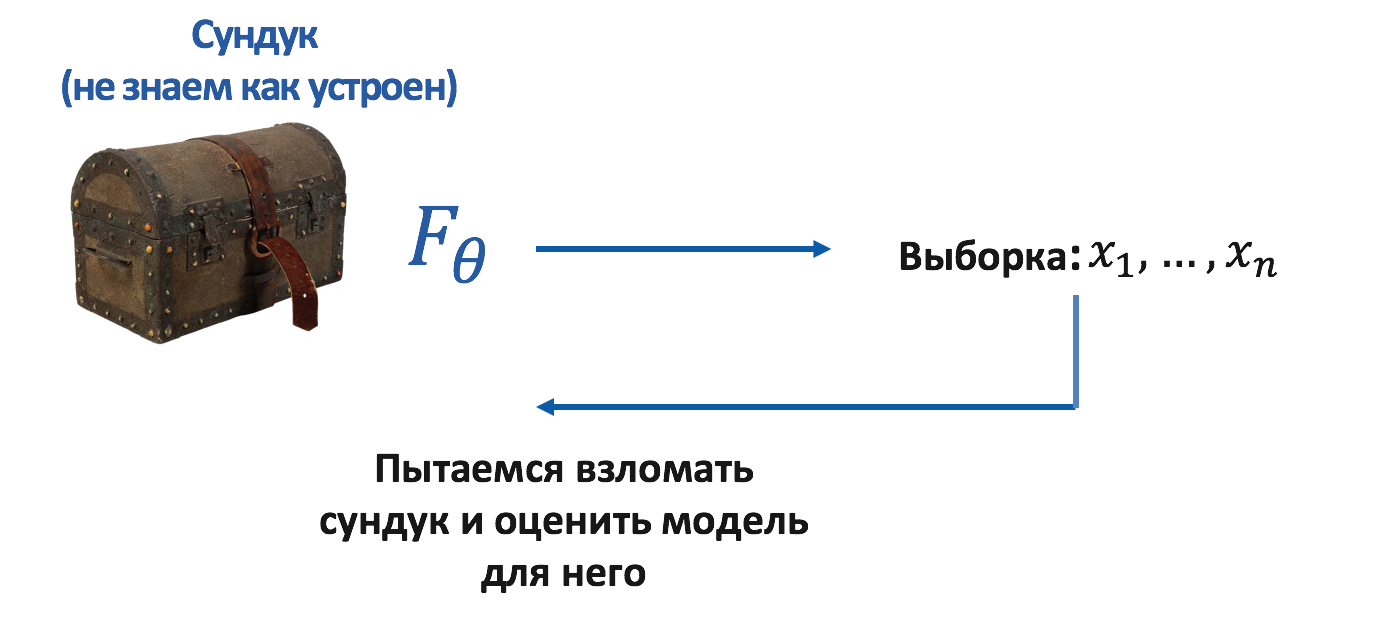
\includegraphics[width=0.85\linewidth]{pic0.png}
\end{center} 

Теория вероятностей занимается тем, что предлагает простейшие модели, которые могли бы описать внутренности сундука. Математическая статистика предлагает кучу способов смотреть на выборки, которые сундук выплюнул. Давайте посмотрим на то, как можно формализовать модель и принять какое-то решение на конкретных примерах. 

\section{Тест Фишера}

На работу нужно взять $8$ человек. Работодатель говорит, что берёт людей на работу абсолютно беспристрастно. Ему неважно какого пола кандидат. Прособеседовались $20$ человек. Из них $8$ были мужчинами, $12$ женщинами. На работу взяли $7$ мужчин и $1$ женщину. Есть ли на рынке труда дискриминация?  

Мы можем попытаться найти ответ на этот вопрос с помощью данных. Предположения, которые можно проверить с помощью данных, называют \indef{гипотезами.} 

Нарисуем табличку. Внизу откладываются суммы по столбцам, справа по строкам. Всего собеседовалось $20$ человек. Эту цифру запишем на диагональке. 

\begin{center}
    \begin{tabular}{|r|c|c|c|}
    \hline
                  & мальчик & девочка &        \\ \hline 
         взяли    &   $7$   &   $1$   & $8$    \\ \hline 
         не взяли &   $1$   &   $11$  & $12$   \\ \hline 
                  &   $8$   &   $12$  & $20$   \\ \hline
    \end{tabular}
\end{center}

Допустим, что работодатель не врёт и отбор правда был беспристрастен. Это наш статус-кво. По-другому статус-кво в статистике называют \indef{нулевой гипотезой.} Чтобы отказаться от нулевой гипотезы нужны весомые доказательства. Какова вероятность получить именно такую выборку, если работодатель не врёт.

Всего вариантов выбрать $8$ человек из $20$ существует $C_{20}^8$ способов. Мы взяли $7$ мальчиков и $1$ девочку. Сделать это есть $C_8^7 \cdot C_{12}^1$ способов. Получается вероятность того, что на $8$ вакансий будет взята только одна девушка составит $\frac{C_8^7 \cdot C_{12}^1}{C_{20}^8} \approx 0.0007$. 

Какова вероятность того, что всё будет ещё хуже и девушек на работу вообще не возьмут? На этот вопрос легко ответить: $\frac{C_8^8 \cdot C_{12}^0}{C_{20}^8} \approx 7 \cdot 10^{-6}$. 

По аналогии можно посчитать все вероятности и нарисовать их на картинке. По оси $x$ отложим число девушек взятых на работу, по оси $y$ вероятность того, что такая ситуация возможна при беспристрастном отборе. В сумме все вероятности будут давать единицу. 

\begin{center} 
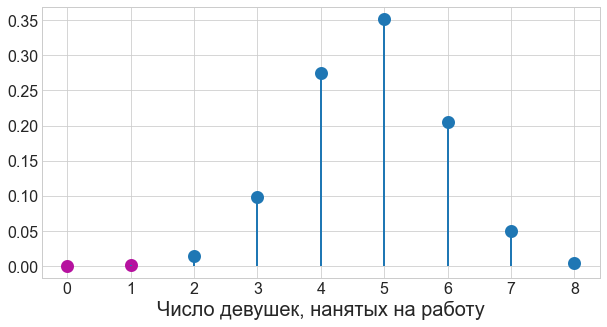
\includegraphics[width=0.7\linewidth]{pic1.png}
\end{center} 

Вероятность того, что при статусе-кво (беспристрастный отбор) мы увидим нашу ситуацию, либо ситуацию ещё хуже оказывается очень низкой. На картинке исходы, которые соответствуют этому, закрашены лиловым. Такую вероятность обычно называют \indef{p-значением (p-value).} 

То, что она оказалась низкой, вовсе не означает дискриминации на рынке труда, но заставляет нас задуматься. Если её нет, то именно такой исход эксперимента, как у нас, должен получаться очень-очень редко. 

Как же принять решение? Обычно для этого выбирают \indef{уровень значимости или ошибку первого рода.} Например, мы можем сказать, что уровень значимости $\alpha = 0.05.$ В эксперименте $p-$значение оказалось меньше него, значит мы не верим в статус-кво и дискриминация на рынке труда действительно есть. 

Уровень значимости - это наша готовность ошибаться и зря отказываться от статуса-кво. Если мы возьмём $\alpha = 0.05$, тогда при постоянном повторении эксперимента, мы в $5\%$ случаев ошибочно откажемся от статуса-кво, потому что при беспристрастном отборе такие редкие события, как в нашем случае иногда происходят. 

Весь смысл этой процедуры заключается в том, что мы хотим мало ошибаться в долгосрочном периоде, при постоянном проведении эксперимента. И она помогает нам обуздать ошибку. 

Кроме ошибки первого рода, уровня значимости, есть ещё и ошибка второго рода. \indef{Ошибка первого рода ---} это когда мы отказались от нулевой гипотезы (статуса-кво), а она была верна. Вероятность такой ошибки обычно обозначают буквой $\alpha$.

\indef{Ошибка второго рода ---} это когда мы остались верны статусу-кво, а он на самом деле неверен. Её вероятность обычно обозначают буквой $\beta$. Удобно нарисовать ещё одну табличку: 

\begin{center}
	\begin{tabular}{|r|c|c|}
	\hline
	                    & $H_0$ верна & $H_0$ не верна \\  \hline 
	выбрали $H_0$       &  ok &    $\beta$ \\      \hline 
	отказались от $H_0$ &   $\alpha$ &  ok \\      \hline 
	\end{tabular}
\end{center}

Ошибка первого и второго рода связаны друг с другом. Когда растёт одна, вторая падает. Жёстко контролировать мы можем только одну из этих ошибок. Вторая минимизируется по остаточному принципу. Для различных критериев можно вывести формулы, которые показывают как эти ошибки связаны друг с другом. Обычно чем больше собрано данных, тем меньше обе ошибки.

На практике обычно не хотят отказываться от статуса-кво. И все мысли формулируют именно так, чтобы было сложно от него отказаться. Например, если тестируют какое-то лекарство, намного страшнее выпустить на рынок плохое лекарство, чем не выпустить хорошее. Из-за этого в качестве гипотезы $H_0$ рассматривают ситуацию, когда новое лекарство бесполезно. Нам нужны весомые статистические доказательства, чтобы отказаться от такого статуса-кво. 

Такой перекос в пользу гипотезы $H_0$ обычно называют \indef{презумпцией нулевой гипотезы.} Это как презумпция невиновности в суде. Нельзя обвинить человека в убийстве, пока это не доказано. С проверкой гипотез всё обстоит абсолютно также.  

Подведём итоги. Наша нулевая гипотеза - на рынке нет дискриминации девушек. Альтернативная гипотеза - дискриминация есть. Если выбрать $\alpha = 0.05$, мы будем вынуждены отвергнуть нулевую гипотезу. Данные говорят против неё.  

Такую процедуру, которая помогает понять взаимосвязаны ли между собой два дискретных признака, пол и найм на работу, называют \indef{тестом Фишера.} 

На самом деле все наши выводы могут оказаться неверны. Мы действовали в рамках конкретной модели. Когда мы строили тест, мы предполагали что есть только два фактора. Вполне возможно, что на самом деле есть какой-то третий признак, который повлиял на эксперимент, а мы его нигде не учли. Возможно, что девушки сами отказались от работы по итогам собеседований, хотя работодатель был готов их взять. 

Когда проводят эксперимент, пытаются исключить все такие третьи факторы из него. Если это оказывается невозможным, либо если эксперимент провести невозможно, приходится привлекать более мощные статистические методы. Например, такой очисткой от лишних зависимостей и попыткой анализа причинно-следственных связей занимается \indef{эконометрика.} 

\section{Критерий знаков}

Президент сказал в новостях, что больше половины квартир стоит дешевле $1$~млн. рублей. Обман ли это? Давайте проверим! Для этого мы можем собрать случайную выборку из квартир. Целых $n$ штук. Будем ставить $+$, если квартира окажется дешевле $1$~млн. Если квартира будет дороже, будем ставить $-$. 

Президент прав, если плюсиков много. Мы изначально верим ему. Это наш статус-кво, наша нулевая гипотеза. Чтобы отказаться от неё, мы должны увидеть в данных что-то ужасное. 

Предположим, что мы посмотрели на $10$ квартир. У нас есть $9$ плюсиков и $1$ минусик. Какова вероятность получить такую выборку либо выборку ещё хуже, при верности нулевой гипотезы? 

\begin{center} 
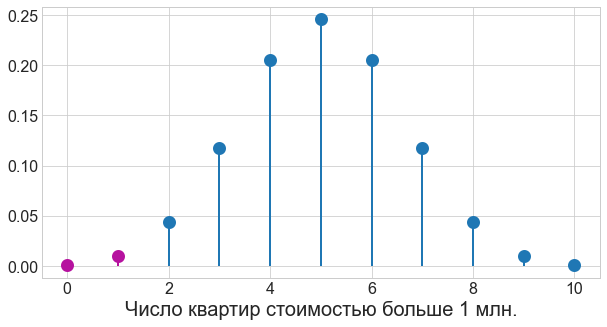
\includegraphics[width=0.7\linewidth]{pic2.png}
\end{center} 

По факту наш эксперимент представляет из себя неправильную монетку. Мы предполагаем, что $p \ge 0.5$. То есть больше половины квартир будут обозначены плюсиками. Альтернатива заключается в том, что $p < 0.5$.  Кратко можно записать это как: 

\begin{equation*} 
    \begin{aligned} 
        &H_0: \quad p \ge 0.5 \\
        &H_a: \quad p < 0.5.
    \end{aligned} 
\end{equation*}

Обычно в таких сложных нулевых гипотезах рассматривают самый шаткий статус-кво и тестируют на верность его. В нашей ситуации таким будет утверждение, что ровно половина квартир оказалась дешевле $1$~млн.

\begin{equation*} 
    \begin{aligned} 
        &H_0: \quad p = 0.5 \\
        &H_a: \quad p < 0.5.
    \end{aligned} 
\end{equation*}

Зафиксируем \indef{уровень значимости} на $\alpha = 0.01.$ Мы можем выбирать его любым. Чем меньше мы его возьмём, тем сильнее мы боимся зря отказаться от статуса-кво по ошибке. При этом ошибки второго рода мы так сильно не боимся. Не надо забывать про её существование. 

Посчитаем \indef{p-значение,} то есть вероятность получить либо наш исход, либо исход ещё хуже при верности статуса-кво: 

$$
pvalue = \frac{10}{2^{10}} + \frac{1}{2^{10}} \approx 0.0107 > \alpha = 0.01.
$$

Получается, что гипотеза о том, что президент не врёт, не отвергается. Многие скажут, что это противоречит здравому смыслу. И будут правы. На самом деле на такой маленькой выборке, при таком маленьком уровне значимости, ошибка второго рода будет зашкаливать. Чтобы сделать её меньше, не меняя ошибку первого рода, можно собрать более большую выборку. Тогда решение будет более устойчивым. 

Такая процедура с расстановкой плюсиков и минусиков называется \indef{критерием знаков}. Её довольно часто используют, когда измерения оказались не очень точными, но при этом нам хочется понять в какую именно сторону направлены изменения. Например, так довольно часто происходит в биологии. 

Если ваши измерения были сделаны точно, то воспользовавшись критерием знаков, вы потеряете довольно много полезной информации, так как превратите все цифры в единицы и нули. В таких ситуациях лучше использовать другие тесты. Например, в будущем мы будем говорить про тесты для средних, основанные на центральной предельной теореме.  

\section{Ранговый критерий (критерий Манна-Уитни)}

Нам срочно нужно протестировать новое лекарство от гипертонии. Для этого мы воспользуемся \indef{двойным слепым тестированием.} В такой ситуации врач не знает, кому что даёт. Пациент тоже не знает, что именно ему дали. 

Если врач знает какие таблетки --- лекарство, а какие --- плацебо, он пытается давать лекарство тем, кто на его взгляд болен сильнее. Это может исказить результат. Поэтому приходится держать врачей в неведении. 

Вопрос заключается в том, есть ли от лекарства какая-то польза. В качестве статуса-кво выберем гипотезу, что никакой пользы нет. Будем давать лекарство людям из группы $A$. Группе $B$ дадим плацебо. У всех людей измерим давление. 

Разбираться в том, есть ли разница между группами будем с помощью следующей процедуры: свалим все наблюдения в одну кучу и отсортируем их по порядку. Каждому наблюдению \indef{припишем свой ранг.} Если все наблюдения разные --- это просто порядковый номер. Если встречаются одинаковые наблюдения, то надо сложить их порядковые номера и поделить на число повторов. 

Пусть в группе $A$ ранги оказались равны $r_1$ и $r_2$. В группе $B$ $r_3, r_4, r_5$. 

\begin{center}
\definecolor{zzttqq}{rgb}{0.6,0.2,0.}
\begin{tikzpicture}[scale=0.8]
\fill[line width=2.pt,color=zzttqq,fill=zzttqq,fill opacity=0.1] (-3.,5.) -- (1.,5.) -- (1.,4.) -- (-3.,4.) -- cycle;
\fill[line width=2.pt,color=zzttqq,fill=zzttqq,fill opacity=0.1] (-3.,3.) -- (3.,3.) -- (3.,2.) -- (-3.,2.) -- cycle;
\draw [line width=2.pt,color=zzttqq] (-3.,5.)-- (1.,5.);
\draw [line width=2.pt,color=zzttqq] (1.,5.)-- (1.,4.);
\draw [line width=2.pt,color=zzttqq] (1.,4.)-- (-3.,4.);
\draw [line width=2.pt,color=zzttqq] (-3.,4.)-- (-3.,5.);
\draw [line width=2.pt,color=zzttqq] (-3.,3.)-- (3.,3.);
\draw [line width=2.pt,color=zzttqq] (3.,3.)-- (3.,2.);
\draw [line width=2.pt,color=zzttqq] (3.,2.)-- (-3.,2.);
\draw [line width=2.pt,color=zzttqq] (-3.,2.)-- (-3.,3.);
\draw (-4,4.8) node[anchor=north west] {\large $A$};
\draw (-4,2.8) node[anchor=north west] {\large $B$};
\draw (-2.5,4.8) node[anchor=north west] {\large $r_1$};
\draw (-0.5,4.8) node[anchor=north west] {\large $r_2$};
\draw (-2.5,2.8) node[anchor=north west] {\large $r_3$};
\draw (-0.5,2.8) node[anchor=north west] {\large $r_4$};
\draw (1.5,2.8) node[anchor=north west] {\large $r_5$};
\draw [line width=2.pt,color=zzttqq] (-1.,5.)-- (-1.,4.);
\draw [line width=2.pt,color=zzttqq] (-1.,3.)-- (-1,2);
\draw [line width=2.pt,color=zzttqq] (1.,3.)-- (1,2);
\end{tikzpicture}
\end{center}

Если получается так, что $r_1 + r_2$ оказалась маленькой, это сигнализирует нам о том, что лекарство помогает и давление понижается. Как понять, как будет распределена такая статистика? 

Предположим, что все наши наблюдения разные. Тогда ранги принимают значения $1,2,3,4,5$. Самое маленькое значение для $r_1 + r_2$ будет равно $1 + 2 = 3.$ Самое большое $5 + 4 = 9$. Посчитаем какую-нибудь из вероятностей. Например, вероятность того, что $r_1 + r_2 = 6.$ Всего два числа из пяти можно выбрать $C_5^2 = 10$ способами. В сумме $6$ можно получить двумя способами. Получается, что $\mathbf{P}(r_1 + r_2 = 6) = 0.2$. По аналогии можно посчитать все другие вероятности. 

\begin{center} 
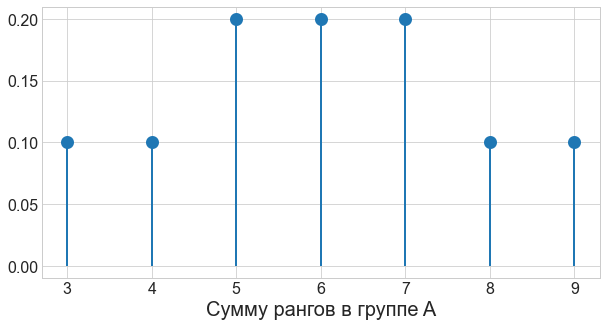
\includegraphics[width=0.7\linewidth]{pic3.png}
\end{center} 

Дальше дело остаётся за малым. Понять насколько наша ситуация плохая и принять решение в соответствии с тем уровнем значимости, который мы выбрали до начала эксперимента. 

Обратите внимание, что в этой задачке мы впервые явно выписали случайную величину, на основе которой мы принимаем решение. Это $T = r_1 + r_2$. В первых двух пунктах можно также выписать такую случайную величину. Для критерия знаков --- это число плюсов. Для критерия Фишера --- это число нанятых девушек. 

Каждый раз мы принимаем решение на основе того, как эта случайная величина себя ведёт при верности нулевой гипотезы. Если она показывает аномальные значения, мы не верим в статус-кво. Такие случайные величины называют \indef{статистиками.} 

В дальнейшем мы будем строить статистические процедуры отталкиваясь от таких величин-помощников. Самое главное --- знать их распределения при статусе-кво. 

Критерий, который мы описали выше, обычно называют \indef{критерием рангов.} В нём мы точно также отказываемся от изначальных измерений, предполагая что они не очень точные. Но в отличие от критерия знаков, мы пытаемся сохранить чуть больше информации, используя вместо плюсов и минусов, порядковые номера измерений.

\section{Схема статистики}

Любое исследование в анализе данных происходит примерно по одной и той же схеме. Сначала у нас есть вопросы. Мы хотим найти на них ответы. Нас может интересовать дискриминация, изменение цен, работоспособность новых лекарств и многие другие вопросы. Чтобы ответить на них, нам надо предположить как именно устроен мир вокруг нас. То есть придумать какую-то модель, которая будет его описывать. 

\begin{center} 
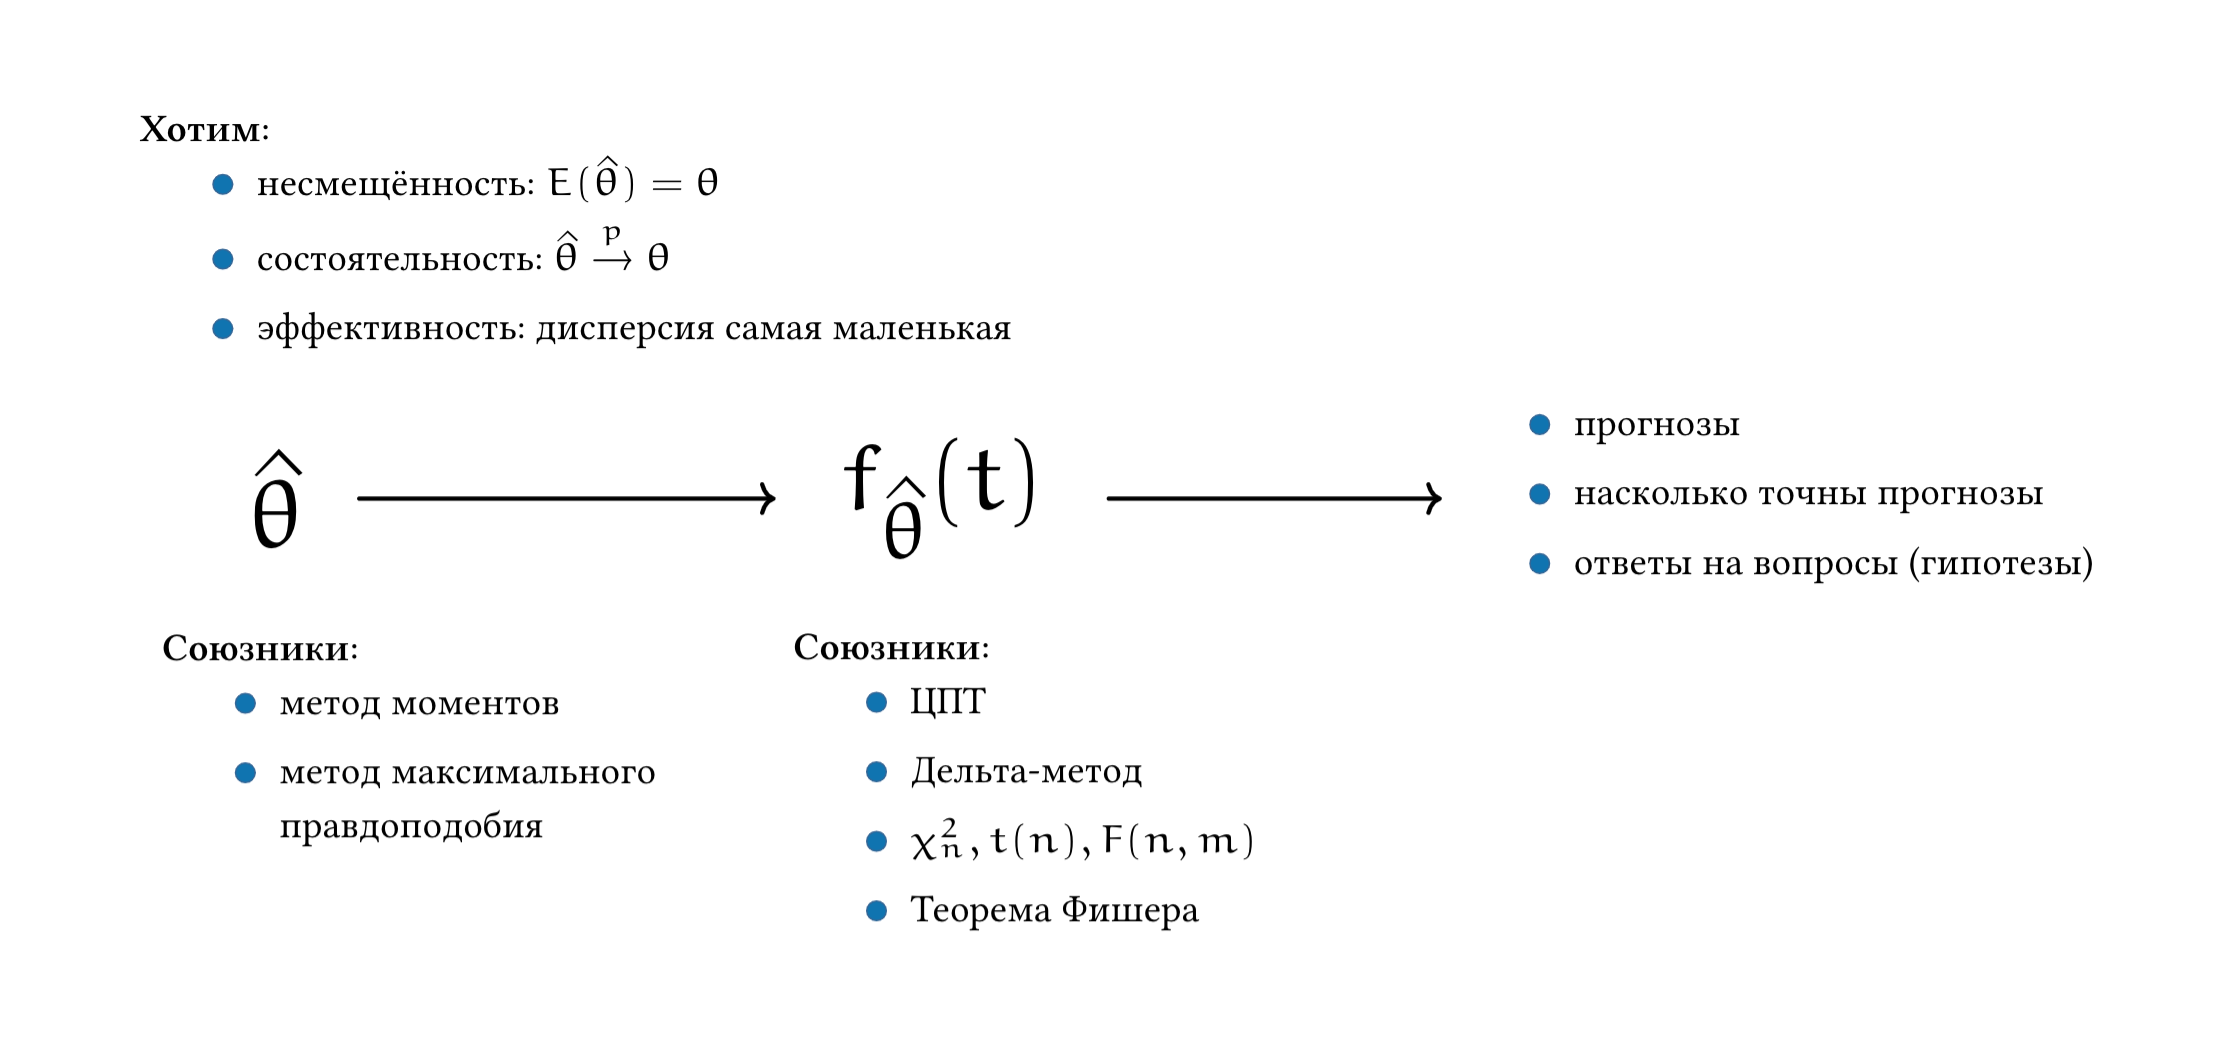
\includegraphics[width=0.99\linewidth]{pic4.png}
\end{center} 

Дальше мир снабжает нас данными. На основе этих данных мы оцениваем неизвестные параметры модели. Есть довольно много методов оценить их. В будущем мы посмотрим на них подробнее. 

Когда у нас есть готовая оценка, нам хочется понимать насколько точной она получилась. Чтобы проверять гипотезы, мы будем строить на её основе статистику. Дальше мы будем смотреть как эта статистика распределена при верности нулевой гипотезы. Если её значение оказывается аномальным, то мы сомневаемся в статусе-кво.

Чтобы понять как именно распределена статистика, обычно используют \indef{союзников --- разные теоремы.} Это может быть центральная предельная теорема или какие-то специфические распределения вроде распределения Стьюдента. Каждая теорема предлагает свой способ отвечать на поставленный перед нами вопрос. 

Например, в трёх критериях выше, мы пользовались дискретными распределениями, которые мы выводили с помощью простейшей комбинаторики. Она была нашим союзником. Никакие параметры в этих распределениях нам оценивать не надо было, достаточно было просто посчитать вероятности. 

Тем не менее, эти критерии очень простые и они игнорируют довольно много информации из выборки. Они слишком упрощают её. Чем больше у модели параметров, тем лучше она может описать данные и тем качественнее может получится ответ на мучающий нас вопрос. Если конечно мы не переобучимся под данные. Но это уже совсем другая история.

Ещё нам часто будет хочется, чтобы оценки неизвестных параметров обладали хорошими свойствами: \indef{немещённостью, состоятельностью и эффективностью.} Методы оценивания придумывают так, чтобы добиваться этих свойств.


\todo[inline]{Написать про расстояния и что мы моделируем именно их}


\section{Какими бывают случайные величины}

Распределения, которые вы изучали на теории вероятностей --- это простейшие варианты таких моделей. Их можно использовать для разных ситуаций. У каждого из них есть параметры, которые описываю его форму. Эти параметры можно оценить по данным. 

\subsection*{Биномиальное распределение}

\indef{Биномиальное распределение} --- дискретное распределение количества успехов среди $n$ испытаний с вероятностью успеха, равной $p$. Обычно записывают как:

$$
X \sim Binom(n, p)
$$

Вероятность того, что произойдёт $k$ успехов расчитывается по формуле: 

$$
\PP(X = k) = {C}^n_k \cdot p^k \cdot (1 - p)^{n - k}, \quad k \in \{0, 1, \ldots, n\}
$$

\textbf{Пример, когда возникает:} сколько раз человек попадёт в баскетбольную корзину при $n$ бросках 

\textbf{Свойства:}

\begin{itemize} 
\item $\E(X) = n \cdot p$
\item $\Var(X) = n \cdot p \cdot (1 - p)$
\end{itemize} 


\subsection*{Распределение Пуассона}

\indef{Распределение Пуассона} --- распределение дискретной случайной величины, представляющей собой число событий, произошедших за фиксированное время, при условии, что данные события происходят с некоторой фиксированной средней интенсивностью $\lambda$ и независимо друг от друга. Хорошо подходит для моделирования счётчиков. Обычно записывают как:

$$
X \sim \Pois(\lambda)
$$

Вероятность того, что произойдёт $k$ событий расчитывается по формуле: 

$$
\PP(X = k) = e^{-\lambda} \dfrac{\lambda^k}{k!}, \quad k \in \{0, 1, \ldots, \}
$$

\textbf{Пример, когда возникает:} число лайков под фотографией, любая случайная величина счётчик, которая подчиняется аксиомам простейшего потока событий

\textbf{Свойства:}

\begin{itemize} 
\item $\E(X) = \lambda$
\item $\Var(X) = \lambda$
\end{itemize} 

\subsection*{Геометрическое распределение}

\indef{Распределение Пуассона} --- распределение дискретной случайной величины, представляющей собой номер первого успеха в серии испытаний Бернулли. Обычно записывают как:

$$
X \sim \Geom(p)
$$

Вероятность того, что номер первого успеха равен $k$ находится как:

$$
\PP(X = k) = p \cdot (1 - p)^{k - 1}
$$

\textbf{Пример, когда возникает:} номер попытки, при которой игрок попал в баскетбольную корзину

\textbf{Свойства:}

\begin{itemize} 
\item $\E(X) = \frac{1}{p}$
\item $\Var(X) = \frac{1-p}{p^2}$
\end{itemize} 


\subsection*{Равномерное распределение}

\indef{Равномерное распределение на отрезке $[a;b]$} обладает плотностью распределения: 

$$
f_X(x) =\begin{cases}
\frac{1}{b - a}, \quad x \in [a; b]  \\
0, \quad x \notin [a; b]
\end{cases}
$$

Обычно записывают как:

$$
X \sim \mU[a; b]
$$

\textbf{Пример, когда возникает:} остаток при округлении чисел

\textbf{Свойства:}

\begin{itemize} 
\item $\E(X) = \frac{a + b}{2}$
\item $\Var(X) = \frac{(b - a)^2}{12}$
\end{itemize} 


\subsection*{Экспоненциальное распределение}

\indef{Экспоненциальное распределение} обладает плотностью распределения: 

$$
f_X(x) =\begin{cases}
\lambda e^{- \lambda x}, \quad x \ge 0  \\
0, \quad x < 0
\end{cases}
$$

Обычно записывают как:

$$
X \sim \Exp(\lambda)
$$

\textbf{Пример, когда возникает:} время между событиями, имеющими распределение Пуассона (время, пока следующий человек придёт в кассу, время до следующего лайка под фото и тп)

\textbf{Свойства:}

\begin{itemize} 
\item $\E(X) = \frac{1}{\lambda}$
\item $\Var(X) = \frac{1}{\lambda^2}$
\end{itemize} 

\subsection*{Нормальное распределение}

Говорят, что у случайной величины $X$ \indef{нормальное распределение с параметрами $\mu$ и $\sigma^2$}, если она обладает плотностью распределения

$$
f_{X}(x) = \frac{1}{\sigma \sqrt{2 \pi}} e^{-\tfrac{(x - \mu)^2}{2\sigma^2}}
$$

Обычно записывают как:

$$
X \sim \mN(\mu, \sigma^2)
$$

\textbf{Пример, когда возникает:} нахождение суммы или среднего большого количества независимых одинаково распределенных величин

\textbf{Свойства:}

\begin{itemize} 
\item $\E(X) = \mu$
\item $\Var(X) = \sigma^2$
\item Если $X \sim \mN(\mu_1, \sigma_1^2)$ и $Y \sim \mN(\mu_2, \sigma_2^2)$, тогда 

$$
a\cdot X + b \cdot Y + c \sim \mN(a\cdot \mu_1 + b \cdot \mu_2 + c, a^2 \sigma_1^2 + b^2 \sigma_2^2) 
$$

\item Для нормального распределения выполняются правила одной, двух и трёх сигм: 

\begin{equation*}
\begin{aligned}
& \PP(\mu - \sigma \le X \le \mu + \sigma) \approx = 0.683 \\
& \PP(\mu - 2\cdot \sigma \le X \le \mu + 2 \cdot \sigma) \approx = 0.954 \\
& \PP(\mu - 3 \cdot \sigma \le X \le \mu + 3 \cdot \sigma) \approx = 0.997
\end{aligned}
\end{equation*}
\end{itemize} 


\subsection*{"Хи-квадрат" распределение}

Пусть случайные величины $X_1, \ldots, X_k$ независимы и одинаково распределены. Причём нормально с параметрами $0$ и $1$. Обычно такой факт записывают следующим образом: 

$$
X_1, \ldots, X_k \sim iid \hspace{2mm} N(0,1).
$$ 

Буквы $iid$ расшифровываются как identically independently distributed (независимы и одинаково распределены).

Случайная величина $Y = X_1^2 + \ldots X_k^2$ имеет \indef{распределение хи-квадрат с $k$ степенями свободы.}  Степень свободы это просто название для параметра распределения.

Обычно записывают как:

$$
Y \sim \chi^2_k
$$   

\textbf{Пример, когда возникает:} на практике тесно связано с выборочной дисперсией для нормальных выборок

\textbf{Свойства:}

\begin{itemize} 
\item $\E(\chi^2_k) = k \cdot \E(X_i^2) = k$
\item $\Var(\chi^2_k) = k \cdot \E(X_i^4) = 2k$
\item Распределение устойчиво к суммированию. То есть, если $\chi^2_k$ и $\chi^2_m$ независимы, тогда $\chi^2_k + \chi^2_m$ = $\chi^2_{k+m}$
\item $\frac{\chi^2_k}{k} \to 1$ по вероятности. 
\end{itemize} 


\subsection*{Распределение Стьюдента}

Пусть случайные величины

$$
X_0, X_1, \ldots, X_k \sim iid \hspace{2mm} N(0,1),
$$ 

тогда случайная величина $$ Y = \frac{X_0}{\sqrt{^{\chi^2_k}/_k}} $$ имеет \indef{распределение Cтьюдента с $k$ степенями свободы.}  
Обычно записывают как:

$$
Y \sim t(k)
$$   

\textbf{Пример, когда возникает:} на практике тесно связано с отношением выборочного среднего и стандартного отклонения нормальных выборок

\textbf{Свойства:}

\begin{itemize} 
\item $\E(Y) = 0, k > 1$
\item $\Var(Y) = \frac{k}{k-2}, k > 2$
\item Симметрично относительно нуля
\item $t(k) \to N(0,1)$ по распределению при $k \to \infty$
\item При $k=1$ совпадает с распределением Коши
\end{itemize} 


\subsection*{Распределение Фишера}

Говорят, что случайная величина 

$$ Y = \frac{^{\chi^2_k}/_k}{^{\chi^2_m}/_m}$$

имеет \indef{распределение Фишера c $k,m$ степенями свободы}.

Обычно записывают как:

$$
Y \sim F_{k,m}
$$   

\textbf{Пример, когда возникает:} на практике тесно связано с отношением выборочных дисперсий двух нормальных выборок

\textbf{Свойства:}

\begin{itemize} 
\item $\E(Y) = \frac{m}{m-2}, m > 2$
\item $\Var(Y) = \frac{2m^2(m + k - 2)}{k (m - 2)^2 (m - 4) }, m > 4$
\item Если $Y \sim F(k,m)$, тогда $\frac{1}{Y} \sim F(m,k)$
\item При $k \to \infty$ и $m \to \infty$ $F(k,m) \to 1$ по вероятности
\item А вот этот факт не раз всплывёт в эконометрике: $t_k^2 = F(1,k)$
\end{itemize} 


\section{Нормальное распределение из воздуха}

\todo[inline]{Вот бы кто-нибудь написал этот раздел!}

\section*{Почиташки} 

\todo[inline]{Сюда список литературы к лекции}


\end{document}